% One-slide talk (1.5 min, poster-style), as required in the seminar. Compile: latexmk -xelatex slide.tex
\documentclass[aspectratio=169,10pt]{beamer}
\usepackage{fontspec}
\usepackage{polyglossia}
\setdefaultlanguage{russian}
\setsansfont{Inter}
\newfontfamily\cyrillicfontsf{Inter}[Ligatures=TeX]
\setmainfont{FreeSerif}
\newfontfamily\cyrillicfont{FreeSerif}[Ligatures=TeX]
\usefonttheme{professionalfonts}
\usepackage{amsmath,amssymb}
\graphicspath{{../figures/}}
\definecolor{ink}{HTML}{1F2328}
\definecolor{accent}{HTML}{1C4FD8}
\definecolor{muted}{HTML}{6B6F76}
\definecolor{tint}{HTML}{EEF2FA}
\setbeamercolor{normal text}{fg=ink}
\setbeamercolor{structure}{fg=accent}
\setbeamertemplate{navigation symbols}{}
\setbeamertemplate{itemize items}{\raisebox{0.15ex}{\scriptsize$\blacksquare$}}
\setbeamersize{text margin left=0.45cm,text margin right=0.45cm}
\newcommand{\x}{\mathbf x}
\newcommand{\G}{\mathbf G}
\newcommand{\hd}[1]{{\color{accent}\bfseries #1}\par\vspace{1pt}}

\begin{document}
\begin{frame}[t]
\vspace{-0.15cm}
{\normalsize\bfseries Вероятностный тензорный поезд как суррогат для байесовской оптимизации\par}
\vspace{1pt}
{\scriptsize\color{muted}Артём Хапилов \quad·\quad научный руководитель: Глеб Рыжаков \quad·\quad github.com/WeCanStart/ptt-bo\par}
\vspace{0.12cm}
\begin{columns}[T,onlytextwidth]
\begin{column}{0.4\textwidth}
\footnotesize
\hd{Задача}
Дорогой чёрный ящик, $N\le200$ вычислений:
$\ \min_{\x\in[0,1]^d} f(\x)$; критерий — регрет $r_N=\min_{i\le N}f(\x_i)-f^*$.\par\vspace{3pt}
\hd{Метод: PTT-EI}
Суррогат вместо гауссовского процесса:\par\vspace{1pt}
\centerline{$g(\x)=\G_1(x_1)\,\G_2(x_2)\cdots\G_d(x_d)$}\vspace{-2pt}
\begin{itemize}\setlength\itemsep{1pt}
\item ядра $\G_k$ — матрицы-функции в базисе Фурье, ANOVA-приор
\item MAP + аппроксимация Лапласа $\Rightarrow\ \mu(\x),\ \sigma(\x)$
\item следующая точка $\x_{t+1}=\arg\max\,\mathrm{EI}(\x)$
\end{itemize}
\vspace{2pt}
\hd{Базовый эксперимент}
11 функций ($d=6$–12), 100 вызовов, 10 сидов. Сравнение с GP-EI, BoTorch LogEI, TuRBO-1, CMA-ES, случайным поиском.
\vspace{4pt}

\colorbox{tint}{\parbox{0.95\linewidth}{\scriptsize\vspace{2pt}
\textbf{Улучшение: TR-PTT} — локальная PTT в доверительной области.
На 9 новых задачах ($d=10$–20): $-1.39$ против $-0.80$ у TuRBO-1, лучше в 75 из 90 пар, $p=2\cdot10^{-10}$.\vspace{2pt}}}
\end{column}
\begin{column}{0.575\textwidth}
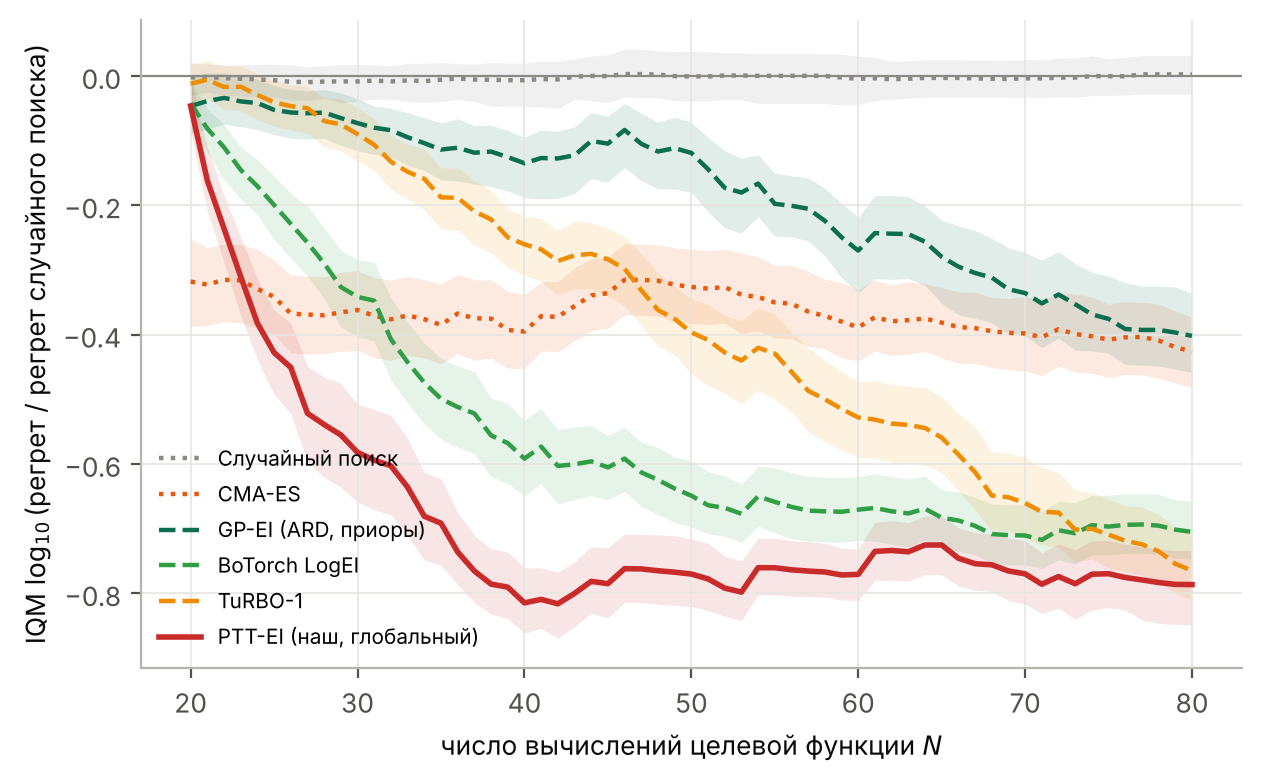
\includegraphics[width=\linewidth,height=4.55cm,keepaspectratio]{e9_anytime.png}\par
\vspace{-1pt}
{\scriptsize\color{muted}Ось $y$: $\log_{10}$ регрета относительно случайного поиска (меньше — лучше), 95\% бутстреп-интервал.\par}
\vspace{2pt}
\footnotesize
\begin{itemize}\setlength\itemsep{1pt}
\item после 40 вызовов PTT-EI лучше всех: $-0.82$ (LogEI $-0.59$, TuRBO $-0.26$)
\item потом застревает: к 100 вызовам TuRBO впереди ($-0.98$ против $-0.86$)
\item выигрыш даёт ANOVA-приор, а не малый TT-ранг функции
\end{itemize}
\end{column}
\end{columns}
\end{frame}
\end{document}
